\section{Results}\label{sec:results}

\subsection{Connected peers}\label{subsec:connected-peers}
\begin{figure*}[!ht]
    \centering
    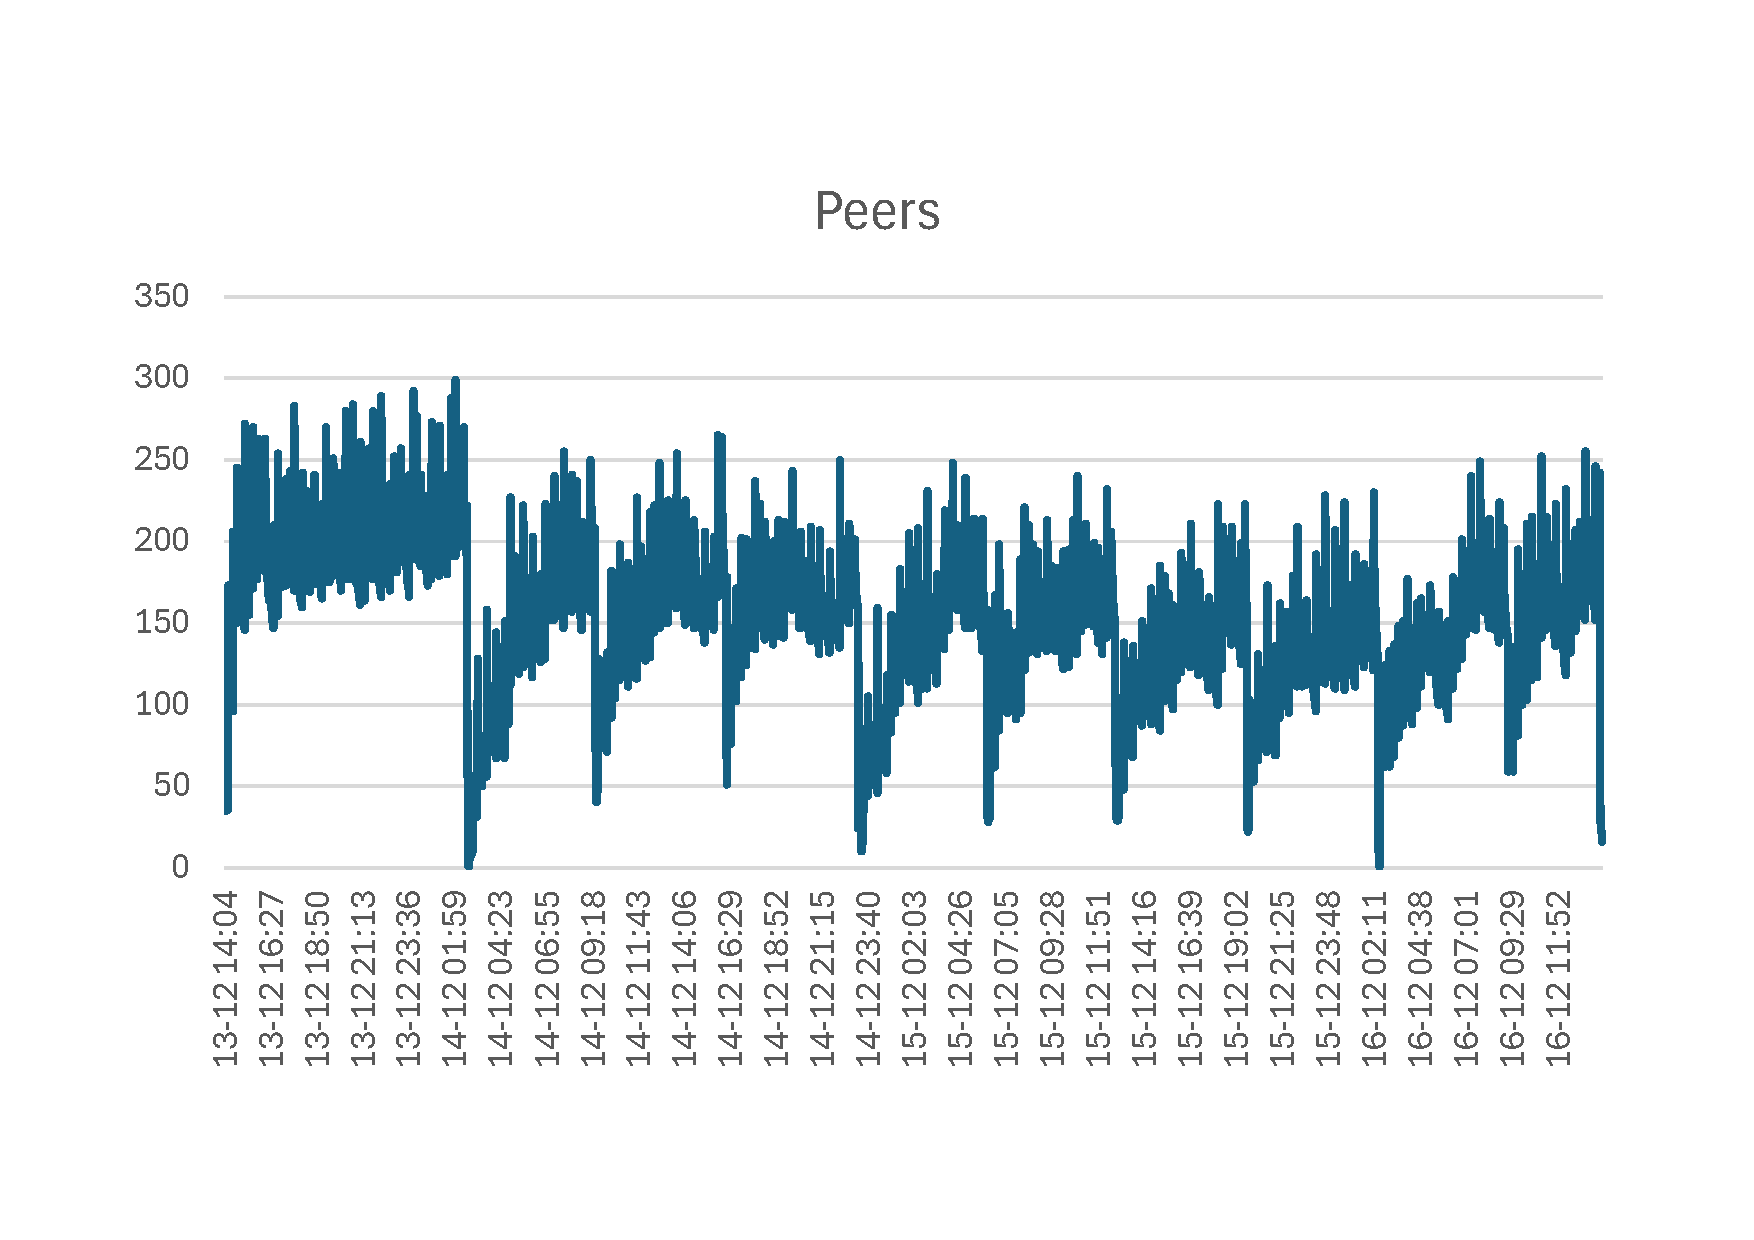
\includegraphics[scale = 0.5]{figures/conPeer2}
    \caption{The number of peers our node was connected to over the time of the experiment.
    Data points are collected every minute and the average amount of peers connected is 148.}
    \label{fig:peersconnected}
\end{figure*}
Throughout the experiment, we kept track of the number of peers our node was connected to.
The number of connected peers is shown in~\autoref{fig:peersconnected}.
Our node was connected to at most 299 peers at once, and the average was 148 peers.
Over the course of the experiment, the number of connected peers fluctuated a lot but would continually rise for the first 12 hours.
Then it would heavily drop and rise again.
This pattern would repeat, but after the first drop it would then drop consistently every 7 hours instead.

\subsection{De-anonymization}\label{subsec:de-anonymization}
Durring the attack we discovered a total of 1,195 unique peers.
The results of the de-anonymization attack are shown in~\autoref{tab:distribution}.
The table showcases the distribution of nodes into the four different categories based on the heuristic described in~\autoref{subsec:inspirational-papers}.
Here we see that 38.661\% the nodes we have encountered have had at least one validator that have been de-anonymized, meaning that the conditions form~\autoref{subsec:inspirational-papers} are fulfilled.
we also see that 5.941\% of the nodes we discovered are subscribed to all 64 subnets.
We did not find any validators on 35.314\% of the nodes we discovered.
This means that we did not receive a single non-backbone attestation from any validator on these nodes.
And lastly we have 20.084\% of the nodes that we discovered that did not fit into any of the other categories.
This could be due to the fact that the node could be hosting a validator, but we could not with enough confidence say that to be the case based on our heuristic.


\begin{table}[]
    \centering
    \begin{tabular}{lll}
        \hline
        & \textbf{Nodes} & \textbf{Distribution} \\ \hline
        \textbf{Deanonymized validators} & 462            & 38.661\%                 \\
        \textbf{64 subnets}              & 71             & 5.941\%                  \\
        \textbf{No validators}           & 422              & 35.314\%               \\
        \textbf{Rest}                    & 240            & 20.084\%                 \\ \hline
        \\
    \end{tabular}
    \caption{Distribution of nodes into the four different categories}
    \label{tab:distribution}
\end{table}


After the attack, we managed to de-anonymize a total of 492,959 validators.
This corresponds to 28\% of the total number of validators in the Holesky network\footnote{As of 2024-01-08 seen on \href{https://holesky.beaconcha.in/}{holesky.beaconcha.in}}.
158,134 of these validators were non-unique, meaning that they had more than one IP-address mapped to them over the durations of the attack.
The results are shown in~\autoref{tab:unique vals}.

In total, we logged 1,183 unique IP addresses.


\begin{table}[]
    \centering
    \begin{tabular}{lll}
        \hline
        & \textbf{Validators} & \textbf{Non-Unique Validators} \\ \hline
        \textbf{Overall} & 492,959             & 158,134                        \\ \hline
        \\
    \end{tabular}
    \caption{Number of validators located by our modified Prysm node. The first column indicates the total number of validators. The second column indicates validators with more than one IP-address mapped to it.}
    \label{tab:unique vals}
\end{table}

\subsection{Validator Distribution}\label{subsec:validator-distribution}
\begin{figure*}[!ht]
    \centering
    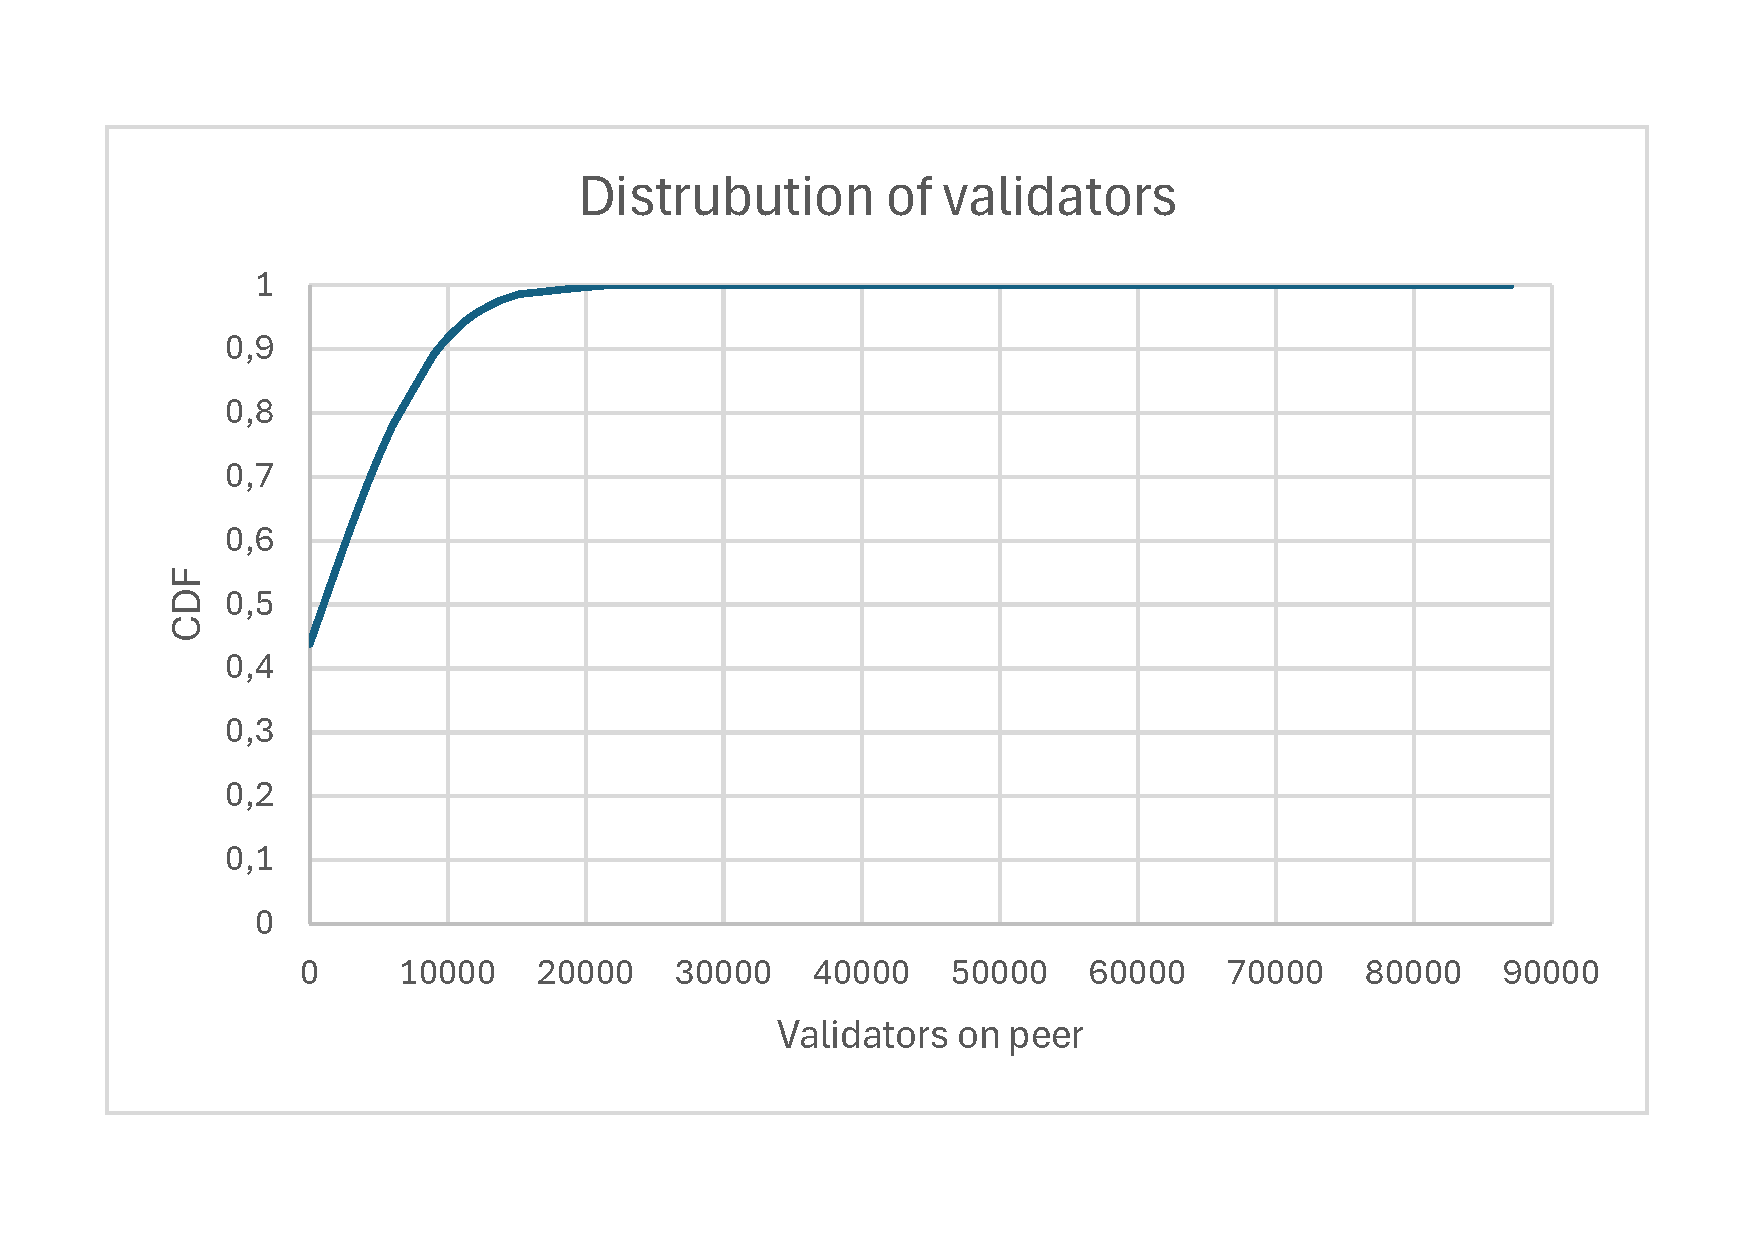
\includegraphics[scale = 0.45]{figures/distval}
    \caption{The cdf showing the distribution of validators on each peer}
    \label{fig:validatorsonpeers}
\end{figure*}
From all the peers we were connected to, we collected the number of validators on each peer.
The cumulative distribution of validators on each peer is shown in~\autoref{fig:validatorsonpeers}.
Here we can see that 57\% of the peers that we connected to have at least one validator.
The amount of validators on each peer ranges from 0 to 87,028, with the average being 1003 validators per peer.
We see that the most common amount of validators on a peer is 1 with about 7\% of the found peers having only one validator.
We also saw that having 110 and 400 were the most common amounts of validators on a peer once we get above 20 validators on a peer.
We found a total of 24 peers that had 10,000 or more validators on them.